\chapter{Theoretical background and Density-based Counting}
\section{Counting overview}
Many approaches have been proposed to resolve the problem of counting in images and videos classified into the following categories: direct approaches, indirect approaches. \\
The direct approaches try to train object detector or object classifier which is used to segment and locate the objects in the images then counting them. Detection or classification is usually made either in the monolithic style or parts-based detection. Monolithic detection approaches train a classifier using features such as Haar wavelets, histogram oriented gradients, edgelet, and shapelet extracted from a full body. Many learning methods such as Support Vector Machines (SVM), random forest, boosting have been used in this approach with varying degree of success. Although successful in low-density crowd scenes, these methods are not likely to produce a good result by the presence of high-density crowds.\\
The indirect approach methods regularly extract several local and global features from groups of objects in the foreground image. The features can be foreground area, or edge count texture features, histograms of edge orientation,  gradient features have been used for encoding low-level information. These methods are more efficient because detecting features are simpler than detecting the whole object. Following features are extracted, a regression function where they learn a mapping between features extracted to their counts.Regression function can be implemented various ways by applying different regression techniques such as linear regression, piecewise.
linear regression, ridge regression, Gaussian process regression and neural network. Foreground features are extracted from foreground segments in a video using standard background subtraction techniques. Blob-based global features such as area, perimeter, perimeter-area ration. Have demonstrated encouraging results. While these methods capture global properties of the scene, local features such as edges and gradient, texture features such as local binary pattern (LBP), histogram oriented gradients (HOG), gray level co-occurrence matrices (GLCM) have been used to further improve the results.
\section{Density-based Counting}
While the above methods were successful in addressing the issues of occlusion and clutter, most of them ignored crucial spatial information as they were regressing on the global count. In opposition, Lempitsky V, Zisserman A \cite{Lempitsky:Zisserman:Destimate} proposed to learn a linear mapping between local patch features and corresponding object density maps. \\
This section starts to explain the density estimation method proposed in \cite{Lempitsky:Zisserman:Destimate} in details and describe the necessary background knowledge to make the thesis relatively self-contained. The work of studying and reimplementing the framework in this section is done by a collaboration between me and my friend, Nguyen Van Luong - ICT 58.
.The order of the subsections follows the processing steps of the system. The first section represents the SIFT feature. Next, the DSIFT features improve from SIFT and how it use in this learning methon. After That, the introduction for k-means and its application in dictionary creation are explained. Finally, the counting method is described in depth. This subsection contains the precise mathematical formula for the problem and how it’s solved by using QP-solver.
\subsection{Feature Representation}

\subsubsection{SIFT}

Matching features across different images in a common problem in computer vision. When all images are similar in nature (same scale, orientation, etc) simple corner detectors can work. But when you have images of different scales and rotations, you need to use the Scale Invariant Feature Transform (SIFT). \\
Scale Invariant Feature Transform (SIFT) is an image descriptor for image-based matching and recognition developed by David Lowe (1999, 2004) \cite{David:sift}. This descriptor as well as related image descriptors are used for a large number of purposes in computer vision related to point matching between different views of a 3-D scene and view-based object recognition. The SIFT descriptor isn't just scale invariant, it's still getting good result when change rotation, illumination, viewpoint. \\
In computer vision, SIFT can use in many way finding interesting point, track images, detect and identify objects.

% \paragraph{Algorithm}

% \begin{enumerate}
%     \item \textbf{Constructing a scale space} This is the initial preparation. Create internal representations of the original image to ensure scale invariance. This is done by generating a "scale space".
%     \item \textbf{LoG Approximation} The Laplacian of Gaussian is great for finding interesting points (or key points) in an image. But it's computationally expensive. So we cheat and approximate it using the representation created earlier.
%     \item \textbf{Finding keypoints} With the super fast approximation, we now try to find key points. These are maxima and minima in the Difference of Gaussian image we calculate in step 2
%     \item \textbf{Get rid of bad key points} Edges and low contrast regions are bad keypoints.  Eliminating these makes the algorithm efficient and robust. A technique similar to the Harris Corner Detector is used here
%     \item \textbf{Assigning an orientation to the keypoints} For each key point calculate an orientation. Any further calculations are done relative to this orientation. This effectively cancels out the effect of orientation, making it rotation invariant
%     \item \textbf{Generate SIFT features} Finally, with scale and rotation invariance in place, one more representation is generated. This helps uniquely identify features
% \end{enumerate}



\subsubsection{Dense SIFT}


While the SIFT descriptor is only calculated at some potential keypoints as presented above, DSIFT computes the SIFT descriptors with a fixed Gaussian window size (octave) at every pixel location. Because of that, DSIFT is slower than SIFT. The density estimation framework uses vlfeat library \cite{VLFeat} for speeding up the DSIFT calculation. The quantization process is applied Euclidean distance \footnote{Euclidean Distance In 'n'-Dimensional Space: 
https://hlab.stanford.edu/brian/euclidean\_distance\_in.html } SIFT feature at each pixel to each word on dictionary. After that, Finding the minimum of distance that calculate before then assign the pixel to the appropriate word of a pre-trained dictionary. The dictionary training is described in the next section.

\subsection{Dictionary Training}
\subsubsection{K-means}

K-means clustering is a kind of unsupervised learning, which is used when you have unlabeled data (i.e., data without defined groups). The goal of this algorithm is to find groups in the data, with the number of groups represented by the variable K. The algorithm works iteratively to assign each data point to one of K groups based on the features that are provided. Data points are clustered based on feature similarity. The results of the K-means clustering algorithm are:
\begin{enumerate}
    \item The centroids of the K clusters, which can be used to label new data.
    \item Labels for the training data (each data point is assigned to a single cluster).
\end{enumerate}

Each centroid of a cluster is a collection of feature values which define the resulting groups. Each centroid is "the center of mass of a geometric object of uniform density", though here, we'll consider mean vectors as centroids.

The initial partitioning can be done in a variety of ways.
\begin{enumerate}
    \item \textbf{Dynamically Chosen} This method is good when the amount of data is expected to grow. The initial cluster means can simply be the first few items of data from the set. For instance, if the data will be grouped into 3 clusters, then the initial cluster means will be the first 3 items of data.
    \item \textbf{Randomly Chosen} Almost self-explanatory, the initial cluster means are randomly chosen values within the same range as the highest and lowest of the data values.
    \item \textbf{Choosing from Upper and Lower Bounds} Depending on the types of data in the set, the highest and lowest (or at least the extremities) of the data range are chosen as the initial cluster means. The example below uses this method.
\end{enumerate}


\subsubsection{Dictionary}
Applying k-means on the DSIFT descriptors collected from the training images to get a dictionary. The words in the dictionary are centroid descriptors of clusters learned by k-means and the number of words in the dictionary corresponds to the number of the clusters which is 256 as per the paper. The dictionary can be trained with just one image or all images in the training set, but using more images will result in a better dictionary.
\subsection{Density Estimation Method}
The overall architecture of the framework consists of 3 main elements: ground truth density images, a feature representation and a learning model.
\subsubsection{Ground Truth Density Images}

Let $I$ is a set of training images which contains $N$ images $I_1, I_2, I_3,...,I_N.$  Having provided a set of 2D points from users’ annotations $P_i={P_1, P_2,..., P_C(i)}$for image $I_i$,  $C(i)$ here is the total number of dot annotations. The density value at each pixel $p$ of image $I_i$ is calculated by the formula:

\begin{displaymath}
    \forall p \in I_i, F^0_i(p) = \sum_{P \in P_i} N(p; P, \sigma^2 1_{2x2})
\end{displaymath}

$N(p; P, \sigma^2 1_{2x2})$ : normalized 2D Gaussian kernel evaluated at p, with the mean at the user-placed dot $P$.\\
From formula above, the integral of all pixels in the image Ii should match the total object counts $C(i)$. However, some objects that are close the image boundary will result in the Gaussian kernel mask being outside of the image and the sum $\sum_{p \in I_i} F^0_i(p)$ is not equal exactly to the total counts $C(i)$. This is acceptable because the partially appeared objects should not be count as a whole.\\
Because the density value of a pixel is the sum of the normalized 2D Gaussian kernel evaluated at p with the mean at the user-placed dot $P$, the pixels whose locations are at the overlapping areas of objects will have high density values and the pixels that are far away from the overlapping areas or the mean $P$ will have smaller values.

\subsubsection{Feture vectors} 

Each pixel $p$ in image $I_i$ is represented by a real-valued feature vector $x^i_p \in R^K$, where $K$ is the number of words in the dictionary. In order to calculate $x_p$, the SIFT descriptor computed with fixed SIFT frame radius (about the size of the cell) and fixed orientation is first extracted at pixel $p$, then it is assigned to a word whose Euclidean distance to the current descriptor is smallest. The assignment is done by setting the dimension of the feature vector corresponding to the order of the word in the dictionary to 1 and the rest dimensions to 0.


\subsubsection{Learning Model}

The Learning model tries to find a vector $w$ that make regression function that can estimate the density of the objects based on their features : \\

\begin{displaymath}
    \forall p \in I_i, F_i(p|w) = w^{T}x^i_p
\end{displaymath}

The function above: 
$w \in R^k$: is vector to be trained from training data. $i$ is index of image, $p$ is pixel in image, $x^i_p$ mean feature vector of pixel in image has index $i$. If Given $w$ the density value of pixel $p$ can be calculate from function $F_i(\bullet|w)$. The remaining problem is find vector $w$ that satisfied minimizes the sum of the differences between the ground truth and the estimated density functions under regularization: 
\begin{displaymath}
    w = \argmin_w\bigg(w^{T}w + \lambda \sum_{i=1}^{N} \mathcal{D}\big(F_{i}^{0}(\bullet),F_{i}(\bullet|w)\big) \bigg)
\end{displaymath}
Where, $\lambda$ is a standard scalar hyperparameter, which is used to control the regularization strength. It is the only hyper-parameter in the framework.
At this point, the problem becomes choosing the distance function $\mathcal{D}$ that best describes the loss to compute the optimal $w$.
Since the parameter vector $w$ depends mainly on the function $\mathcal{D}$, selecting the appropriate function will have a huge impact on the framework performance. Naturally, one can easily come up with the ideas of choosing the distance function to be one of two following functions:
\begin{itemize}
    \item The function $\mathcal{D}$ can be some function of $L_P$ metric such as the $L_1$ metric (sum of absolute per-pixel differences) or the $L_2$ metric (sum of squared per-pixel differences). This kind of functions makes the above formula a standard regression problem in which each pixel in the training images provides a training sample for the problem. However, this choice is not suitable for the loss function because this type of functions does not associated directly with the real quantity the framework care about which is the total number of objects in images.
     \item Because of the limitation of the first distance function, the absolute or the squared difference between the overall sums over the whole images could be chosen as $\mathcal{D}$. The selection fits the final goals of learning to count. However, many annotated images are required for training if this choice is used because spatial information in the annotation is discarded.
\end{itemize} 
Due to the disadvantages of both choices, the paper proposes another distance function called the MESA distance. For an image $I$, the definition of MESA distance $\mathcal{D}_{MESA}$ between two functions $F_{1}(p)$ and $F_{2}(p)$ on the pixel grid is the largest absolute difference between sums of $F_{1}(p)$ and $F_{2}(p)$ over all box subarrays in $I$:

\begin{displaymath}
    \mathcal{D}_{MESA}(F_{1}, F_{2}) = \max_{B \in \textbf{B}} \bigg\lvert \sum_{p \in \textbf{B}}F_{1}(p) - \sum_{p \in \textbf{B}}F_{2}(p) \bigg\rvert
\end{displaymath}

Where, $B$ is the set of all box subarrays of image $I$.

\begin{center}
    \begin{figure}
        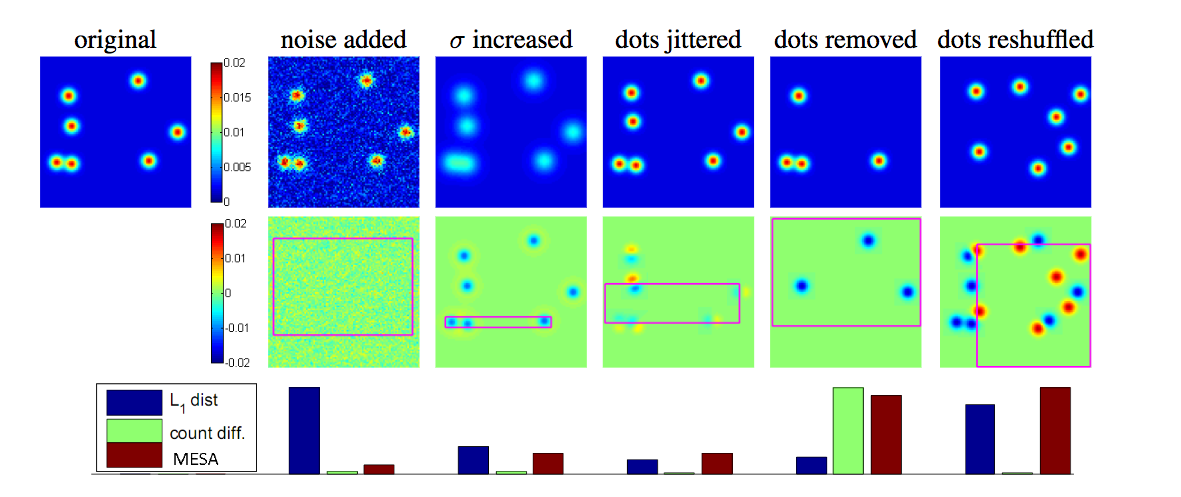
\includegraphics[width=\textwidth]{Chapters/Fig/mesa}
        \caption{Comparison of Distances for Matching Density Functions}
        \label{fig:mesa}
    \end{figure}
\end{center}

In figure \ref{fig:mesa}, the top-left image show ground truth density for a set of dot. The top row is the densities obtained by applying some perturbations on the original one. In the middle row shows the per-pixel differences in each comparison, the red rectangle in this row is the boxes which has the largest absolute difference as defined in the MESA distance formula. The comparisons of the per-pixel $L_1$ distance, the absolute difference of overall counts, and the MESA distance between the original and the perturbed densities are placed at the bottom row.\\
The comparisons of three distance functions show that the MESA distance tolerates the local modifications (noise, change of Gaussian kernel), but reacts heavily to the change in the number of objects or their positions.\\
There are several advantages when using MESA distance in the counting framework. Firstly, Since the set of all subarrays include the full image, $\mathcal{D}_{MESA}$ gives an upper bound on for the absolute differences of the overall count estimates given by the two densities $F_1$ and $F_2$. Secondly, $\mathcal{D}_{MESA}$ between the two density functions that differ by a zero-mean high-frequency signal or an independent zero-mean noise is small because the sum of positive and negative deviations of $F_1$ and $F_2$ pixels tend to be small over the large regions. Finally, $\mathcal{D}_{MESA}$ is sensitive to the overall spatial layout of the densities. In other words, if the counts of two densities are equal, but the layout of them are different, the MESA distance will be large.\\
The $\mathcal{D}_{MESA}$ is rewritten for it can be compute efficiently :
\begin{displaymath}
    \mathcal{D}_{MESA}(F_{1},F_{2}) = \max\bigg( \max_{B \in \textbf{B}}   \sum_{p \in B}{\big(F_{1}(p) - F_{2}(p)\big)},  \max_{B \in \textbf{B}} \sum_{p \in B}{\big(F_{2}(p) - F_{1}(p)\big)} \bigg)
\end{displaymath}
From above equation we can compute $\mathcal{D}_{MESA}$ by find max of inner maxima that involes solving 2D maximun subarrays problem. That problem is finding the subarray of a given 2D array with the largest sum. There are several solutions to solve this problem, but the simplest of the efficient ones is perform an exhaustive search over all boxes in image with dynamic programming. \\

The learning problem can be rewritten as a convex quadratic program:
\begin{center}
    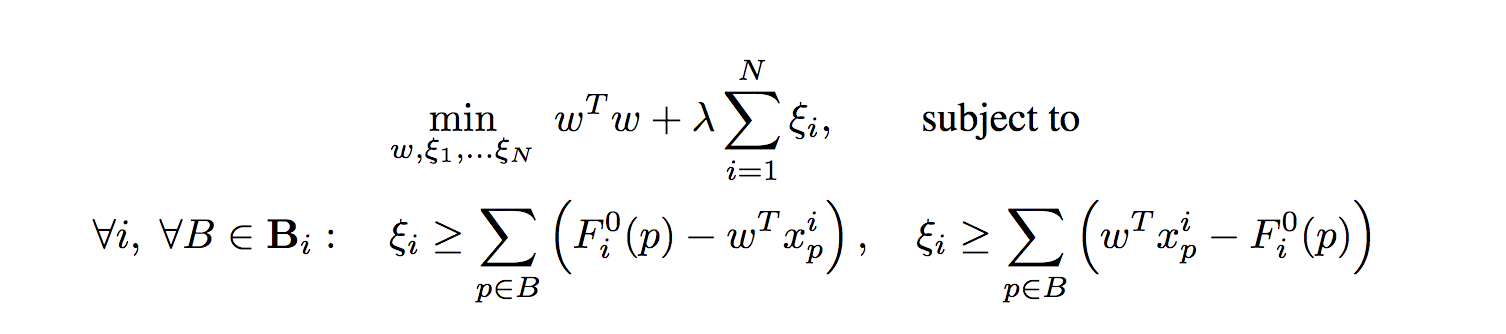
\includegraphics[width=\textwidth]{Chapters/Fig/learningeq}
\end{center}

Where,$\xi_i$ is the auxiliary slack variable of image $i$
$B_i$ is the set of all subarrays in image $i$.\\
When the above optimization reaches the optimum, the optimal vector $\hat{\omega}$ is found and the slack variables equal the MESA distance. However, we cannot directly apply a QP-solver to the optimization because the number of linear constraints is combinatorial. To address this problem, a small subset of constraints (20 boxes as per the paper) is activated first. The optimization problem is solved with that set of active constraints in an iterative manner. For solution $^j$ in iteration j, the solution $^{j}\omega$,$^{j}\xi_1$,...,$^{j}\xi_N$ is then used to find the boxes that violate the constraints most. Those boxes have the largest differences between the ground truth density and the estimated density. In other words, they are the 2D maximum subarrays of $F^{0}_{i}(\bullet) - F^{0}_{i}(\bullet|^{j}\omega)$ and $F^{0}_{i}(\bullet|^{j}\omega) - F^{0}_{i}(\bullet)$ respectively. The iterations terminates when the sums of maximum subarrays in all images are smaller or equal to $^{j}\xi_{i}.(1+ \epsilon)$. The value of is added so that the convergence can be reached after a small number of iterations. The convergence must approximate the global minimum and therefore should be small ($<<1$).\\
\textbf{Algorithm}\\
\textbf{For} from 1 to 20:
    \begin{itemize}
        \item Draw random box and assign to random image in training set 
        \item Calculate count of that box from ground truth density over the random box 
        \item get feature \& weight of that box
        \item add that feature \& ground truth density \& weight \& box to constraints of QP-Solver
    \end{itemize}
\textbf{For iteration} from 1 to \textbf{maxIteration}:
    \begin{itemize}
        \item Run QP-Solver after that get slacks \& $\omega$
        \item Estimate density with $\omega$ for each image
        \item In each image get difference value between current density and ground truth density 
        \item In each image Find the most violate box with the difference value calculate in previous step
        \item In each image add difference value \& true count of that box \& that box to constraints of QP-Solver.
    \end{itemize}

The last $\omega$ is our models.
